\documentclass[12pt]{article}

\usepackage{a4wide}
\usepackage[colorlinks=true,linkcolor=black,urlcolor=blue,bookmarksopen=true]{hyperref}
\usepackage{bookmark}
\usepackage{fancyhdr}
\usepackage[utf8]{inputenc}
\usepackage[T1]{fontenc}
\usepackage{graphicx}
\usepackage{float}
\usepackage[a4paper,headheight=16pt,scale={0.7,0.8},hoffset=0.5cm]{geometry}
\usepackage{caption}
\captionsetup[figure]{font=small,labelfont=small}


\pagestyle{fancy} % Encabezado y pie de página
\fancyhf{}
\fancyhead[L]{Federico Brasburg - 96653}
\fancyhead[R]{Trabajo Final - Simulación}
\renewcommand{\headrulewidth}{0.4pt}
\fancyfoot[C]{\thepage}
\renewcommand{\footrulewidth}{0.4pt}

\begin{document}
\begin{titlepage} % Carátula
	\hfill
\includegraphics[width=6cm]{images/logofiuba.jpg}
    \centering
    \vfill
    \Huge \textbf{Simple Model of Spiking Neurons}
    \vskip2cm
    \Large Trabajo Final - Simulacion \\
    Facultad de ingenieria\\ % Curso 1 para el de la tarde y 2 para el de la noche
    \vskip2cm
    \begin{tabular}{ | l | l | } % Datos del alumn
      \hline
      Alumno: & Brasburg, Federico \\ \hline
      Número de padrón: & 96653 \\ \hline
      Email: & federico.brasburg@gmail.com \\ \hline
    \end{tabular}
    \vskip2cm
    \vfill
    \vfill
\end{titlepage}

\tableofcontents % Índice general
\newpage

\section{Absctract}\label{sec:intro}
El objetivo de este trabajo es del replicar los resultados obtenidos en Simple Model of Spiking Neurons - Izhikevich(2003). \cite{paperOriginal} (a partir de ahora llamado "paper original").
El paper original presenta un modelo que tiene la capacidad de reproducir comportamientos conocidos de las neuronas corticales, como por ejemplo el \textit{spiking} (una traducción bastante desafortunada seria disparada)
o el \textit{bursting} (cuando hay muchos disparos). El modelo propuesto combina la plausibilidad biológica de las dinámicas de Hodgkin–Huxley \cite{HodgkinHuxley} y la eficiencia computacional de las neuronas de integración y disparo.
Estas ultimas neuronas son las que se utilizan para generar modelos de Machine Learning. Usando el modelo propuesto se puede simular miles de neuronas corticales de disparo con una resolución de 1ms utilizando cualquier PC (personal computer).
Por fuera del paper original, se probó el modelo propuesto con diferentes parámetros.
\\ \\
Palabras clave: Bursting, Hodgkin–Huxley, PCNN, neuronas de integración y disparo, spiking, corteza cerebral.
\newpage
\section{Introducción}
Para entender como funciona el cerebro humano, se necesita combinar estudios experimentales sobre sistemas nerviosos de animales y humanos con simulaciones numericas de gran escala de modelos cerebrales.
Al momento de desarrollar modelos de neuronas spiking, se tienen siempre dos requerimientos que son aparentemente mutualmente excluyentes sobre cada neurona:
\begin{enumerate}
    \item Tienen que ser computacionalmente simples
    \item Tienen que tener la capacidad de producir patrones de disparos mostrados por neuronas biológicas reales.
\end{enumerate}

Usar modelos que sean biofisicamente semejantes a los de Hodgkin–Huxley es computacionalmente imposible, ya que solo se pueden simular muy pocas al mismo tiempo en tiempo real. Por el otro lado, usar un modelo
puramente con neuronas que integren y disparen es muy efectivo computacionalmente pero es totalmente irrealista y es incapaz de generar las dinámicas de las neuronas reales como el spiking o el bursting.

En el paper original, se presenta un modelo simple de spiking que es bilogicamente plausible al de Hodgkin–Huxley y es computacionalmente eficiente como el de integración y disparo.
El modelo propuesto solo toma 4 parámetros y con eso solo es capaz de reproducir los comportamientos de spiking, bursting y muchos mas conocidos de neuronas corticales reales. En la Fig 1 se puede observar
algunos comportamientos conocidos reproducidos en la corteza cerebral de una rata. \\ \\

\newpage

\begin{figure}
    \centering
        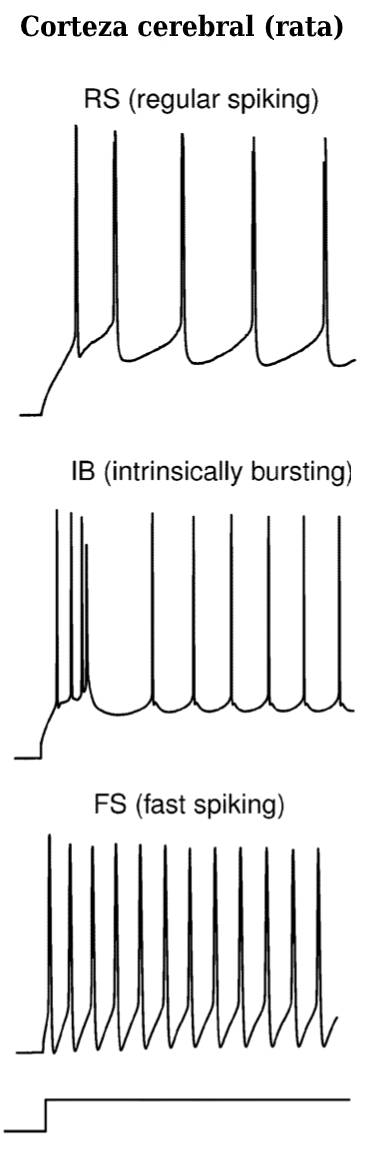
\includegraphics[height=10cm]{images/rata.jpg}
    \caption[fontsize=2pt]{Imagen obtenida del paper original. Se pueden apreciar tres comportamientos conocidos como lo son el regular spiking (RS), el intrinsically bursting (IB) y el fast spiking (FS) en la corteza de una rata}
\end{figure}

El modelo completo fue publbicado por primera vez en \cite{modeloPrimero} en una forma trigonometrica. En este paper se presenta en una forma mas adecuada para simulaciones a gran escala

\section{El Modelo}
Las metodologias de bifurcacion \cite{bifurcacion} nos permiten reducir el modelo neuronal de Hodgkin-Huxley a un sistema bidimensional de ecuaciones diferenciales ordinarias:
\begin{equation}
    \frac{dv(t)}{dt} = 0.04 v(t)^2 + 5 v(t) + 140 - u(t) + I\\
\end{equation}
\begin{equation}
    \frac{du(t)}{dt} = a(b v(t) - u(t))
\end{equation}
Ademas, a $(1) \ y  \ (2)$ le agregamos la regla:
\begin{equation}
    Si \ v(t) >= 30 mV,\ entonces \
        v(t) = 30 \ y \ u(t) = u(t) + d
\end{equation}
Los parámetros del sistema son $a, b, c \ y \ d$. $t$ es el tiempo. \\ \\

La variable $v(t)$ representa el potencial de la neurona (medido en mV) y $u(t)$ representa la variable de recuperacion de la neurona,
que cuenta las activaciones de los iones $K^{+}$ y la desacativacion de los $Na^{+}$, ademas aporta negativamente a $v(t)$ \\

Se dice que sucede un \textit{spike} cuando $v(t)$ es mayor a 30mV. Luego de un spike, el voltaje de la membrana ($v(t)$) y la variable de recuperacion ($u(t$)) son reiniciadas de acuerdo a $(3)$.
A cada neurona la estimula una corriente sinaptica, distinta para cada neurona, que se ve representada en el sistema de ecuaciones en la variable $I$ (que puede ser una funcion dependiente del tiempo o constante).

La parte de $0.004v(t)^2 + 5v(t) + 140$ fue obtenida adecuando las dinámicas del inicio de un spike de una neurona cortical, por lo que mV es la escala para $v(t)$ y $ms$ para el tiempo.
El potencial de reposo (cuando un spike no esta sucediendo) ronda los -70 y -60 mV dependiendo del valor de $b$. Como la mayoria de las neuronas reales, el modelo no tiene un limite de potencial fijo (llamamos limite al voltaje del cual parte un spike).
Dependiendo del historial de spikes de la neurona el potencial limite podria ser tan bajo como -55 mV o tan alto como -40 mV.
Los parámetros tienen los siguientes significados:
\begin{itemize}
    \item El parámetro $a$ describe la escala de tiempo para la varible de recuperación ($u(t)$), por lo que un $a$ chico va a ser que la recuperación de un spike sea mas lenta. Un valor normal es $a = 0.02$
    \item El parámetro $b$ describe la sensitividad de la variable de recuperación a la fluctiación del limite de potencial de la membrana. Mayores valores de $b$ acoplan a $v(t)$ y a $u(t)$ fuertemente dando como resultado
posibles oscilaciones de sublimites y dinámicas de spiking con un limite bajo. Un valor normal es $b = 0.2$. El caso $b < a$ corresponde a una bifurcacion saddle-node del estado de reposo \cite{modeloPrimero}
    \item El parámetro $c$ es el valor que se le asigna al potencial de la membrana ($v(t)$) luego de un spike. Un valor normal es el de $c = -65 mV$.
    \item El parámetro $d$ es el valor que se le agrega a la variable de recuperacion ($u(t)$) luego de un spike. Un valor normal es el de $d = 2$.
\end{itemize}

Distintas combinaciones de parámetros resultan en distintos patrones intrinsecos de disparos, incluidos los conocidos de las neuronas corticales ya mencionados y de las neuronas talamicas (del talamo).
Una posible extension del modelo propuesto es el de tratar $u(t), a$ y $b$ como vecores y usar $\sum{u}$ en lugar de $u$ para el voltaje. Esto sirve para tener en cuenta conductancias lentas con multiples esccalas de tiempo, pero el autor del paper considera que esta extensión es innecesaria para las neuronas corticales.

\section{resolución de la ecuacion diferencial}

Esta es una sección que no es parte del paper original pero me parecio importante de contar como hice las simulaciones. Para comenzar se intentó resolver el sistema de ecuaciones diferenciales con python con la libreria $simpy$ \cite{Sympy}
pudiendo llegar a una solucion para ambas
ecuaciones ($v(t)$ y $u(t)$). Se utilizó el sistema original del paper y se tomo como condiciones iniciales las del reset luego de un spike para ambas funciones.
Pero se presentó la dificultad de que dicha solución tambien tenia que tener en cuenta la regla $(3)$ del sistema original, lo cual resultó imposible e hizó que se tenga que buscar otra solución. \\ \\
Finalmente, se adoptó como solución una encontrada utilizando la definición de derivada. La definición es la siguiente: \\
\begin{equation}
    f'(x) = \lim_{h \to 0} \frac{f(x + h) - f(x)}{h}
\end{equation}
\\
Luego se aproximó de la siguiente manera utilizando el metodo de Euler \cite{Euler}:
\begin{equation}
    f'(x) \approx \frac{f(x + h) - f(x)}{h}
\end{equation}

Finalmente se utilizó $(5)$ para obtener las siguientes funciones ($h$ es la resolución del sistema, en este caso va a ser 0.1ms):
\begin{equation}
    v(t + h) \approx h(0.04 v(t)^2 + 5 v(t) + 140 - u(t) + I) + v(t)
\end{equation}
\begin{equation}
    u(t + h) \approx h(a(b v(t) - u(t))) + u(t)
\end{equation}

Se puede apreciar claramente que dichas ecuaciones no son la solución al sistema de ecuaciones diferenciales. Lo unico que proveen es: partiendo de valores iniciales $v_0$ y $u_0$,
se puede obtener la serie de valores $u_0,...,u_n$ y $v_0,...,v_n$. Para simular solo se necesita de dichas series, no es necesaria la función solución, por lo que se dió como aceptable dicha resolución.

\section{Diferentes tipos de dinámicas}

La siguiente sección habla sobre los distintos patrones que se ven en las neuronas, vale la pena destacar que cada simulación se realizó con los valores
mencionados en el paper original y resolución de (0.1 ms). \\

Las neuronas neocorticales del cerebro mamifero pueden ser clasificadas en diferentes tipos de acuerdo al patron de spiking y bursting visto en estudios intracelulares. \\

\subsection{Celulas corticales exitatorias}
Todas las celulas corticales exitatorias pueden ser divididas en tres clases \cite{firingPatters} \cite{chatteringCells}:

\newpage
\subsubsection{Regular spiking (RS)}
Las neuronas de tipo \textit{Regular spiking} (Disparos regulares, a partir de ahora RS) son las neuronas mas comunes del cortex cerebral. Cuando se le aplica un estímulo prolongado en el tiempo (como en la realizacion de esta simulación)
dispara algunas veces (entre 2 y 4 veces) con un periodo entre disparos pequeño y luego el periodo incrementa (dich comportamiento se puede apreciar en al figura 2). Esa transición entre periodos entre disparos se llama \textit{adaptacion de frecuencia de disparos}.
Si se incrementa la intensidad del estimulo entonces aumenta la la frecuencia de disparos (figura 3), aunque tiene un limite la frecuencia (no puede tender a infinito) por el tiempo de recuperacion de la neurona.
Para generar este tipo de neuronas los parámetros del modelo corresponden a $c = 65$ mV (teniendo en cuenta que
es el voltaje utilizado para el reset de la neurona, es muy bajo) y $d=8$.

\begin{figure}[h]
    \centering
        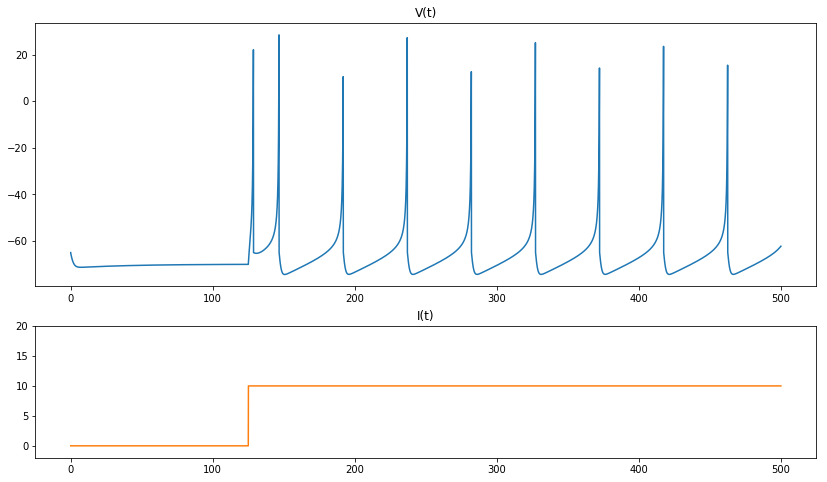
\includegraphics[height=8cm]{images/RS_I10.png}
    \caption[fontsize=2pt]{Imagen simulada con los parámetros del paper. Se puede ver el fenomeno descripto anteriormente, al principio con un periodo pequeño entre disparos y luego aumenta.}
\end{figure}

\begin{figure}[h!]
    \centering
        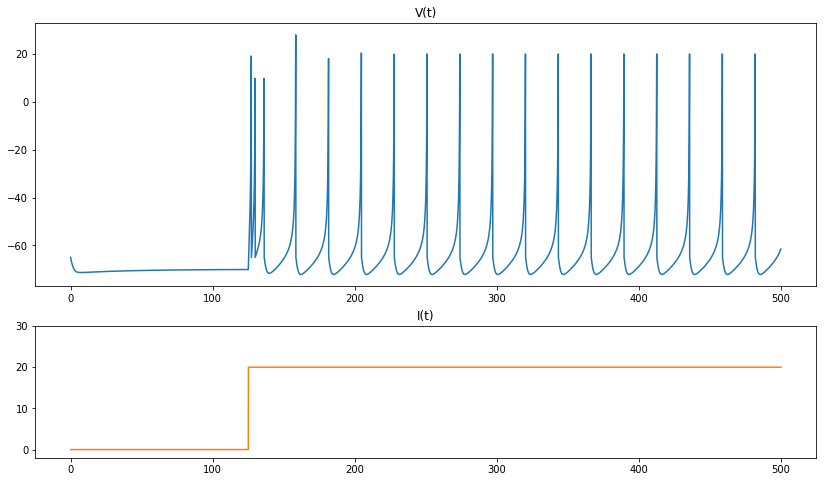
\includegraphics[height=8cm]{images/RS_I20.png}
    \caption[fontsize=2pt]{Imagen simulada con los parámetros del paper con un estimulo el doble de intenso. Se ve que al duplicar la intensidad del estimulo la frecuencia de disparos aumenta}
\end{figure}
 \newpage

\subsubsection{Intrinsically bursting (IB)}

Las neuronas de tipo \textit{Intrinsically bursting} (estallido intrinseco, a partir de ahora IB)
disparan un clasico estallido de disparos al comenzar a recibir el estimulo seguido luego de repetidos disparos unicos con una frecuencia constante (figura 4).
En el modelo, esta neurona se corresponde a los siguientes parámetros: $c = -55 mv$ (alto voltaje para el rest) y $d = 4$ (salto grande de $u$ luego de un disparo).
Durante el estallido inicial $u(v)$ va creciendo hasta que eventualmente cambia la dinámica de los disparos para pasar de estallidos a disparos regulares. \\


\begin{figure}[h!]
    \centering
        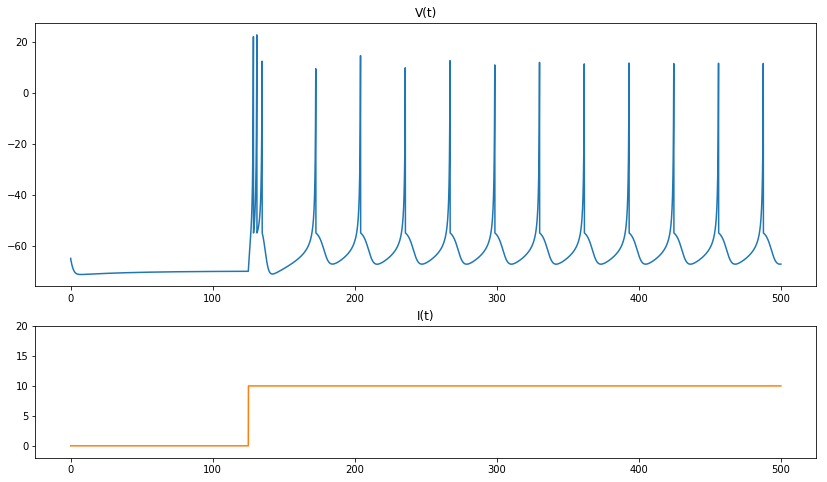
\includegraphics[height=8cm]{images/IB.png}
    \caption[fontsize=2pt]{Imagen simulada con los parámetros del paper para la neuronas tipo IB. Se vislumbra claramente el estallido inicial seguido de disparos regulares}
\end{figure}
\newpage

 \subsubsection{Chattering (CH)}

 Las neuronas de tipo \textit{Chattering} (parloteo, a partir de ahora CH) disparan estallidos clásicos de disparos separados por muy poco espacio (figura 5). A diferencia de las IB, este tipo de neuronas solo dispara estallidos, en ningun momento dispara disparos regulares del estilo RS.

 \begin{figure}[h!]
    \centering
        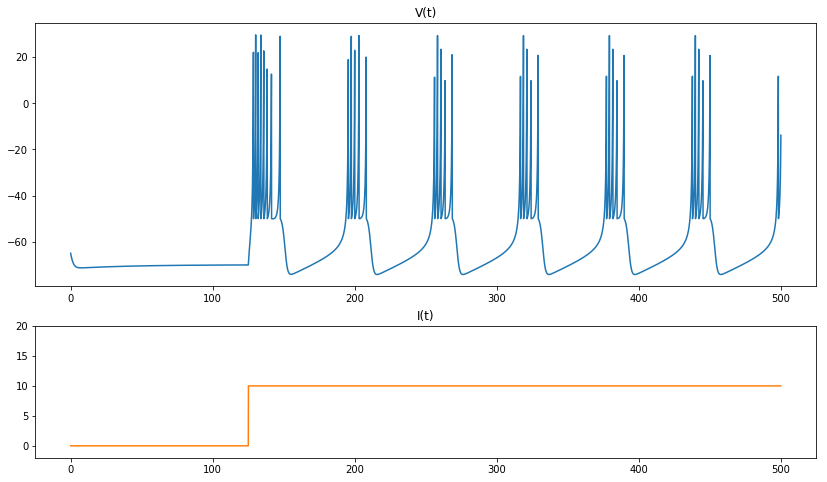
\includegraphics[height=8cm]{images/CH.png}
    \caption[fontsize=2pt]{Imagen simulada con los parámetros del paper. Se pueden ver los estallidos mencionados en el paper}
\end{figure}

Los parámetros del modelo para CH se corresponden a $c = -50$ mV (un voltaje muy alto para el reset) y $d = 2$ (un salto de $u$ moderado luego de cada disparo).

\subsection{Celulas corticales inhibitorias}
Todas las celulas corticales inhibitorias pueden ser divididas en las siguientes dos clases \cite{inhibitorias}:

\subsubsection{Fast spiking (FS)}
Las neuronas de tipo \textit{Fast spiking} (disparos rapidos, a partir de ahora FS) pueden disparar trenes de disparos con una frecuancia extremedamente alta sin practicamente periodo de adaptación.
Para esta neurona el paramentro que hay que modificar es $a = 0.1$ para una rapida recuperación.

\begin{figure}[h!]
    \centering
        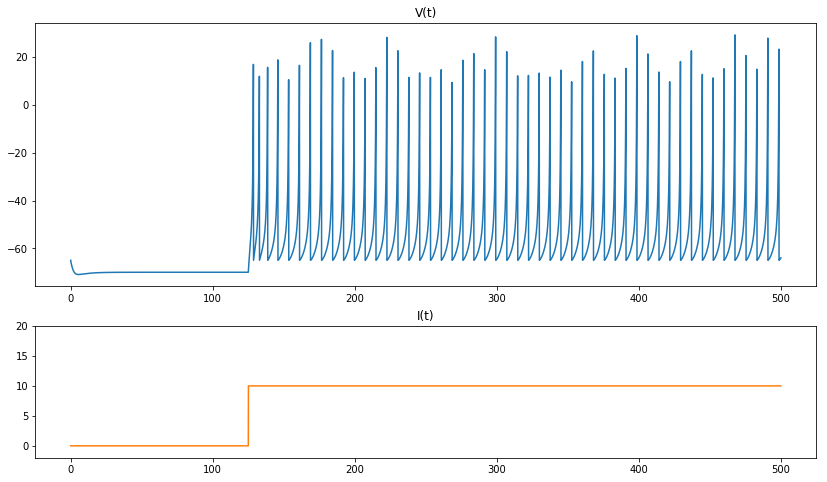
\includegraphics[height=8cm]{images/FS.png}
    \caption[fontsize=2pt]{Imagen simulada con los parámetros del paper para la neuronas tipo FS. Se pueden ver la alta frecuencia (constante) de disparos}
\end{figure}

\subsubsection{Low threshold spiking}
Las neuronas de tipo \textit{Low threshold spiking} tambien pueden disparar trenes de disparos de alta frecuencia pero con una notable adaptacion de la frecuencia de disparo. Estas neuronas tienen un limite (threshold)
de disparo bajo que se logra adaptando el parámetro $b$ seteandolo en $0.25$

\begin{figure}[h!]
    \centering
        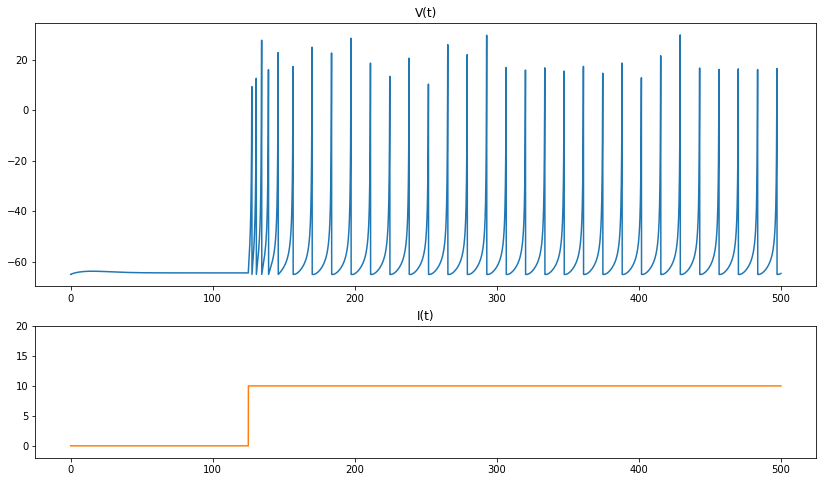
\includegraphics[height=8cm]{images/LTS.png}
    \caption[fontsize=2pt]{Imagen simulada con los parámetros del paper para la neuronas tipo LTS. Debido al limite bajo, se ve una simulacion semejante a la de neuronas FS}
\end{figure}
\newpage

\subsection{Otros tipos de neuronas}
El modelo puede tamien reproducir otros tipos interesantes de dinámicas

\subsubsection{Thalamo-cortical (TC)}
Las neuronas de tipo \textit{Thalamo-cortical} (thalamo-corticales, a partir de ahora TC) tienen dos tipos de regímenes de disparos:
Cuando estan en reposo (el potencial ronda los $-60 mV$) y luego son despolarizadas, exhibiendo disparos tónicos semejantes a los de una neurona RS (figura 8). \\
Por otro lado, si se entrega un estimulo de corriente negativo para que el potencial de membrana se hiperpolarice (con un voltaje semejante a $-90 mV$), la neurona dispara un estallido como una neurona (IB) (figura 9).
Es importante mencionar que en este segundo caso el estimulo tiene que empezar con un estimulo negativo ($-10mV$) y luego dejar de estimular, al dejar de estimular se reproduce el estallido.

\begin{figure}[h!]
    \centering
        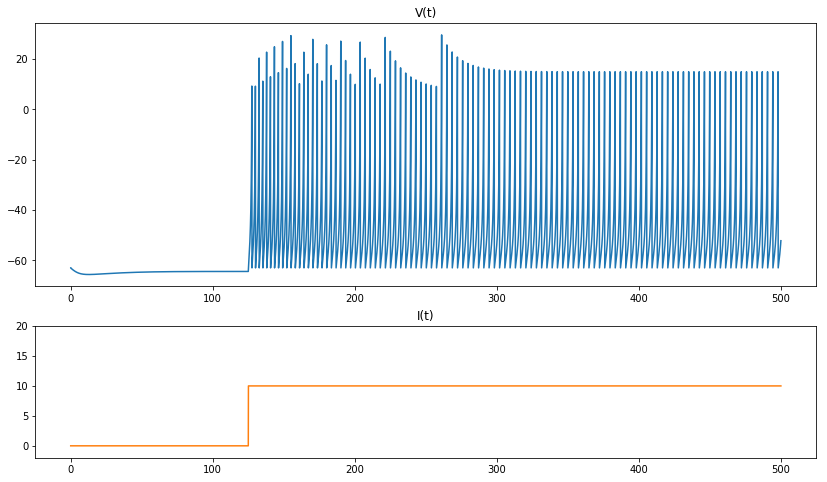
\includegraphics[height=8cm]{images/TC_normal.png}
    \caption[fontsize=2pt]{Imagen simulada con los parámetros del paper para la neuronas tipo TC sin hiperpolarización. Se ve un comportamiento semejante a una RS pero con una frecuencia de disparo alta}.
\end{figure}
\newpage

\begin{figure}[h!]
    \centering
        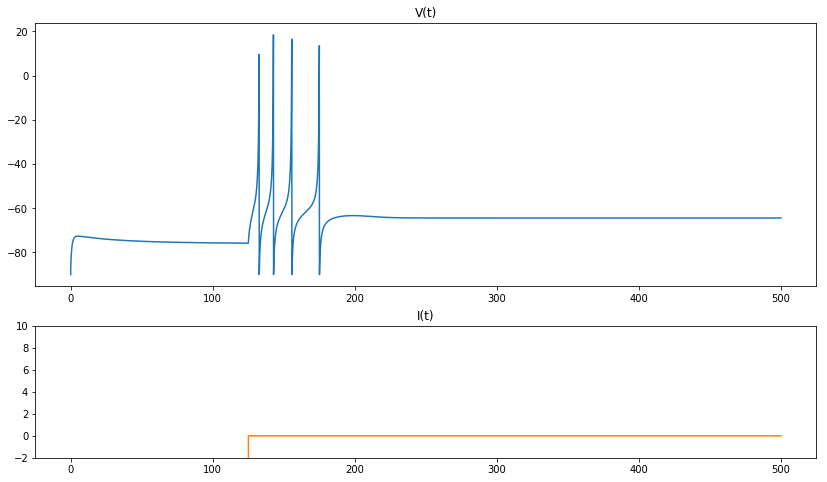
\includegraphics[height=8cm]{images/TC_hiper.png}
    \caption[fontsize=2pt]{Imagen simulada con los parámetros del paper para la neuronas tipo TC con hiperpolarización. Se ve que al dejar de estimular negativamente se producen algunos disparos y luego no sucede nada mas}.
\end{figure}
\newpage

\subsubsection{Resonator (RZ)}
Las neuronas de tipo \textit{Resonator} (resonadoras, a partir de ahora RZ) tienen oscilaciones subliminales amortiguadas. Estas neuronas resuenan a entradas rítmicas que tienen la frecuencia apropiada.
Este comportamiento correspende a $a = 0.1$ y $b = 0.26$. \\
Es interesante notar que hay una biestabilidad de los estados de reposo y RS: la neurona puede cambiar entre los estados por estímulos breves adecuadamente programados.

\begin{figure}[h!]
    \centering
        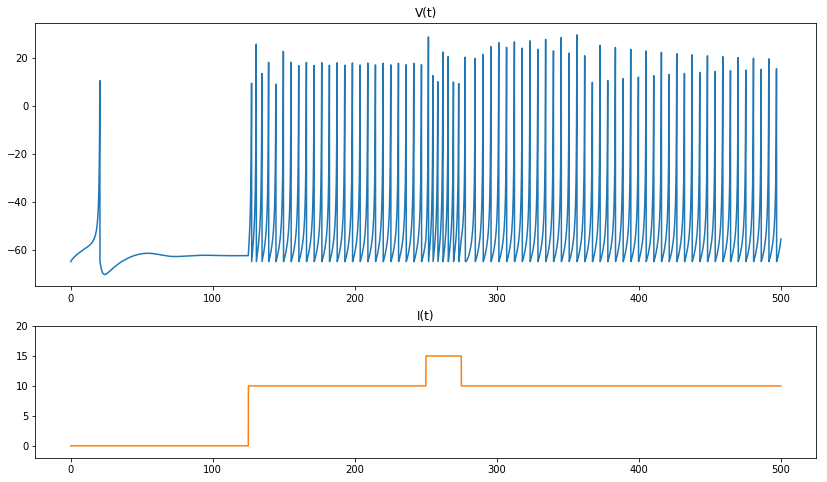
\includegraphics[height=8cm]{images/RZ.png}
    \caption[fontsize=2pt]{Imagen simulada con los parámetros del paper para la neuronas tipo RZ. Se puede ver que con el inicio de los estimulos cambia la frecuencia de disparos}.
\end{figure}

\subsection{conclusiones sobre dinámicas de neuronas}

Otras dinámicas de neuronas pueden tambien ser descriptas por el modelo presentado en el paper, como por ejemplo las de hipocampo, las de los ganglios basales, las de tronco encefalico, etc. \\ \\
En el paper original tambien se menciona que la ecuación (1), especificamente la parte de $0.04 v(t)^2 + 5 v(t) + 140$, del modelo propuesto se justifica para simulaciones de gran cantidad de neuronas en simultaneo.
Si se tiene interes en el comportamiento de una sola neurona, existe otras opciones de la funcion mas adecuadas. Por ejemplo la ecuación $0.04 v(t)^2 + 4.1 v(t) + 108$ con un parámetro $b = -1$ es una mejor opción para la simulación de neuronas RS, por que
estos parámetros llevan a un saddle-node en una birfucación de circulo y una exitacion de clase 1. \cite{saddleNode}

\section{Simulación de pulso acoplado}
El paper menciona que este modelo fue usado para correr una red de 10000 neuronas corticales de disparos con 1000000 conecciones sinapticas en tiempo real con resolución de 1ms en una computadora de escritorio de 1Ghz.
Luego se propone un código en matlab que simula una red de 1000 neuronas conectadas aleatoriamente en tiempo real. \\ \\
Con la idea de replicar la corteza cerebral de los mamiferos, se eligió que la relación entre neuronas exitatorias comparado a las inhibitorias sea de 4 a 1 y que las conecciones inhibitorias sean mas fuertes que las exitatorias (casi el doble de fuertes).
Ademas de las entradas sinapticas (de las otras neuronas), cada neurona recibe estimulacion thalamica. \\

En principio, se podrian usar celulas RS para modelar todas las celular exitatorias y FS para modelar todas las inhibitorias. Para lograr esto de manera hetereogenea (para que diferentes neuronas tengan diferentes dinámicas)
se asignaron los parámetros $a, \ b, \ c \ y \ d$ correspondietes a las FS y RS pero agregandoles un compomente aleatorio. \\
Para las células exitatorias se asignó:
\begin{itemize}
    \item $a_i = 0.02$
    \item $b_i = 0.2$
    \item $c_i = -65 + 15 * r^2$
    \item $d_i = 8 - 6 * r^2$
\end{itemize}

Siendo $r_i$ una variable aleatoria uniformemente distribuida en $[0,1 ]$. $i$ es el indice de la neurona. De esta manaera si $r_i = 1$ corresponderia a una neurona CH y si $r_i = 0$ corresponderia a una RS.\\
\\
Para las células inhibitorias se asignó:
\begin{itemize}
    \item $a_i = 0.02 + 0.08 * r_i$
    \item $b_i = 0.25 - 0.05 * r_i$
    \item $c_i = -65$
    \item $d_i = 2$
\end{itemize}

El modelo creado corresponde a la clase de redes neuronales de pulso acoplado (PCNN).
\newpage
\subsection{Modelo usado para las simulaciones}
Si bien el código propuesto en el paper esta escrito en lenguaje $MatLab$ \cite{MatLab}, para la simulación de la red de este paper se utilizó en lenguaje $Python$ \cite{Python}.
Se realizó en un lenguaje distinto por distintos motivos. Primero se consideró que tendria mas valor intentar replicar una simulación en un lenguaje distinto al propuesto en el paper
para mostrar una correcta apreciación del modelo (y del código) original. Se tuvo que aprender $MatLab$ para luego poder hacerla simulación en código $Python$ \\
Por otro lado, el diseño del código implementado en $Python$ es muy distinto al original, se intento hacer un diseño totalmente orientado a objectos y mucho mas extensible para otras futuras pruebas y simulaciones.
El código original no era muy claro y era bastante pobre en cuanto a buenas prácticas de programación, lo que hacia que fuese bastante dificil cambiar los parámetros (o agregar nuevos) para futuros experimentos.

\subsection{Simulación}
El paper original toma una consideración a la hora de ejecutar la simulación que es la de normalizar los disparos. Lo que propone es que cuando el voltaje de la neurona supera el umbral para ser reseteada (30mV), se setea el voltaje en 30mV (en lugar de hacer el reset directamente) y luego en el siguiente instante de tiempo se hace el reset. Esta consideración la menciona en la descripción de la imagen del resultado obtenido pero no la implementa en el código.
Lo que se hizo para replicar la simulación es hacer el experimento dos veces: una con la consideración del paper orginal y otra sin la misma.

\begin{figure}[h!]
    \centering
        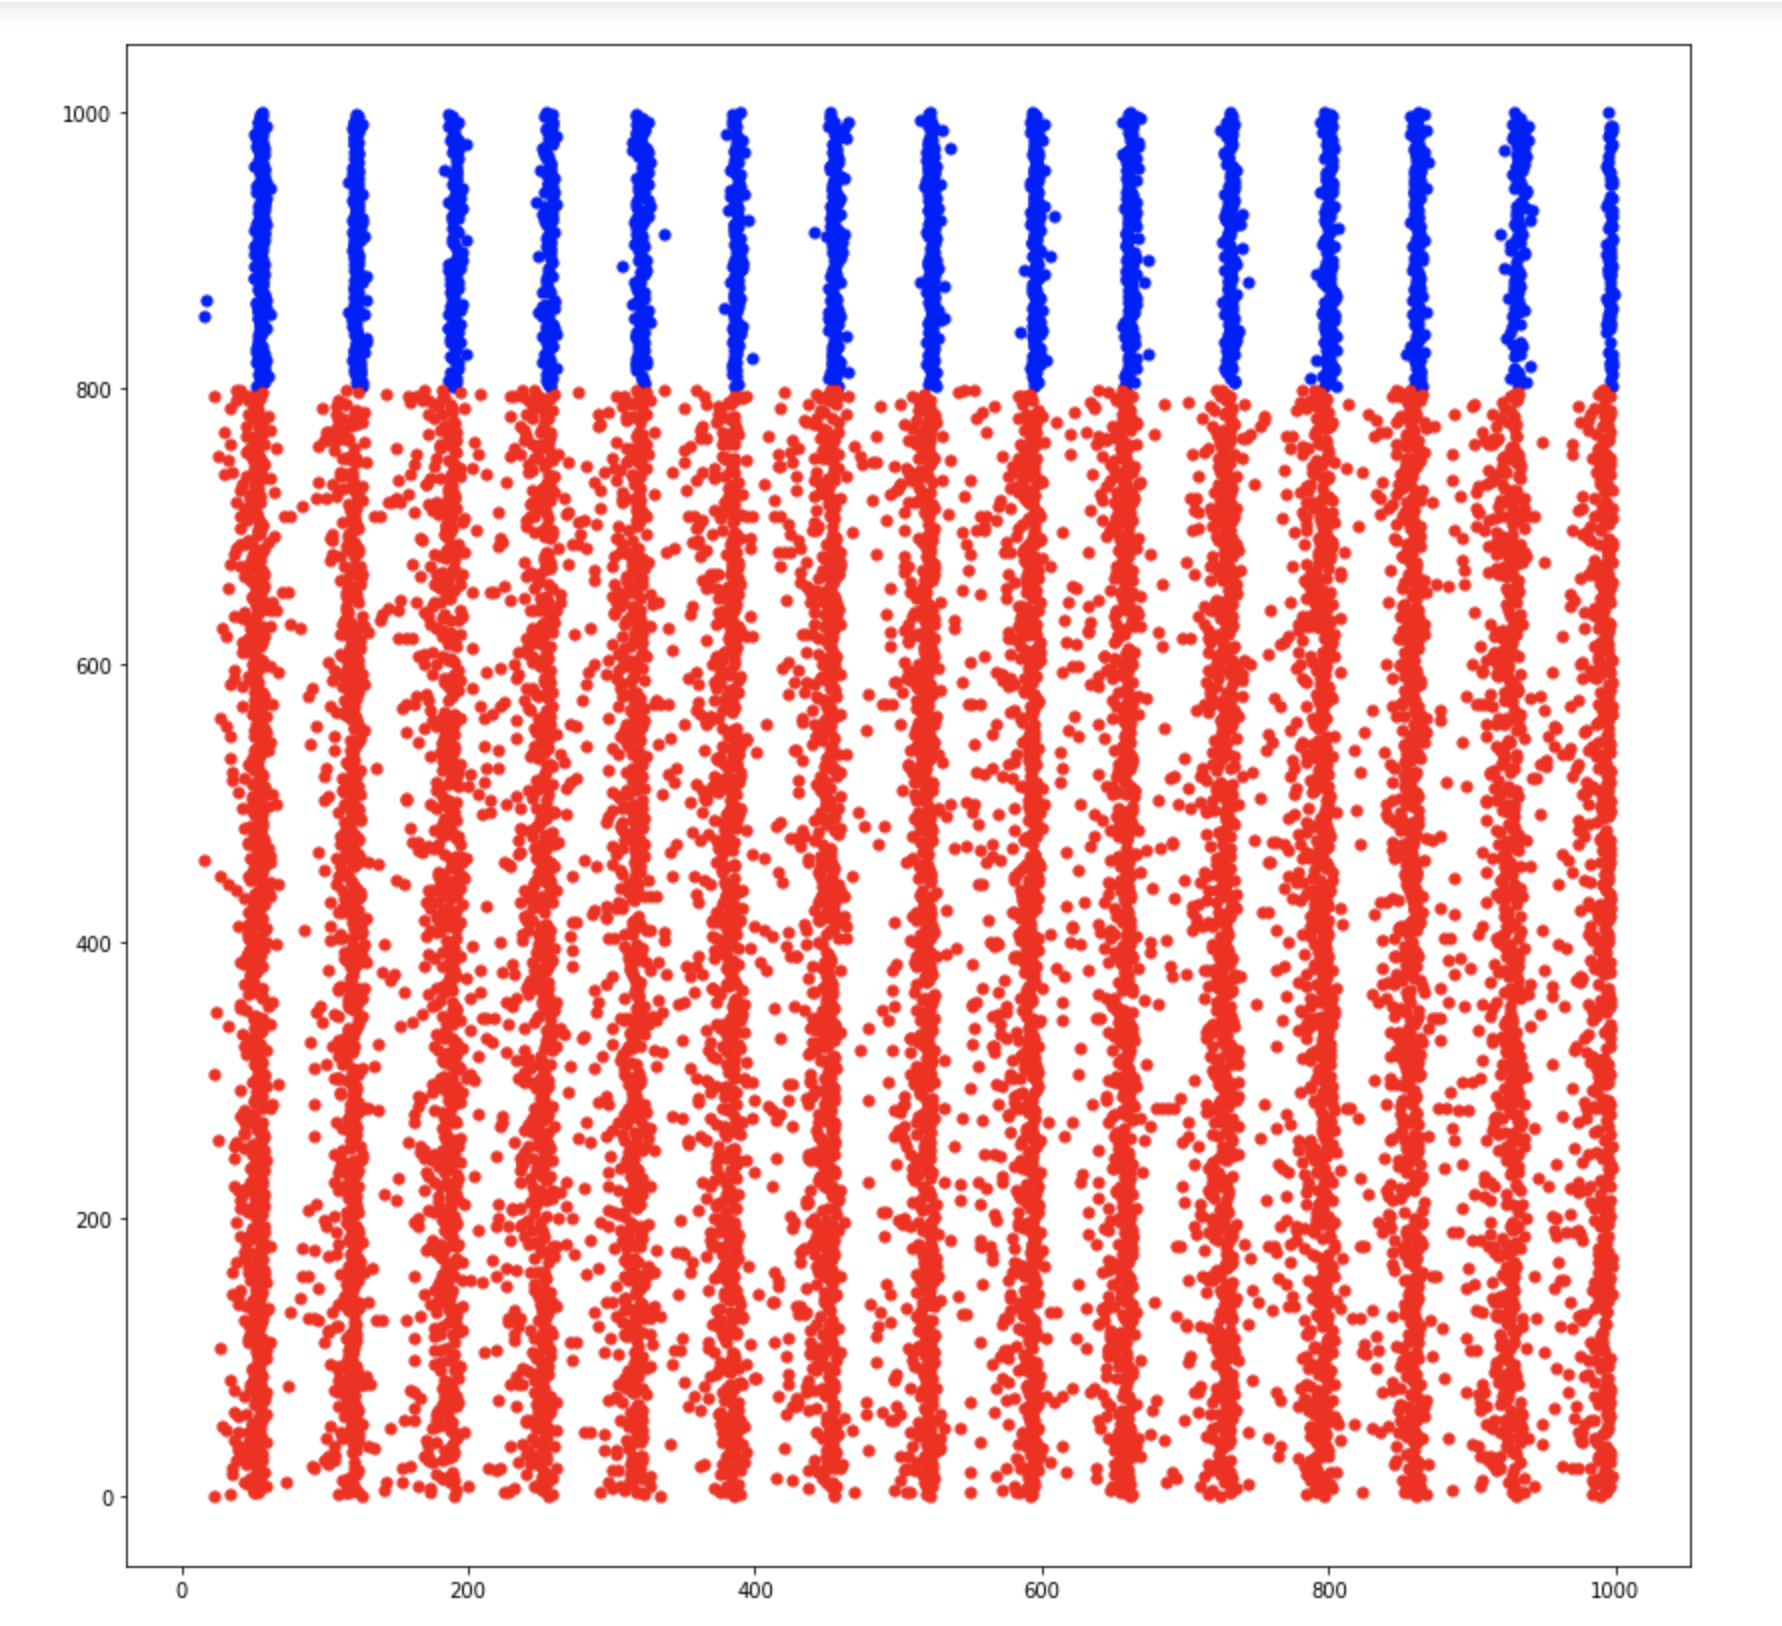
\includegraphics[height=8cm]{images/resultadoConNorm.png}
    \caption[fontsize=2pt]{Resultado obtenido con la consideración}.
\end{figure}

\begin{figure}[h!]
    \centering
        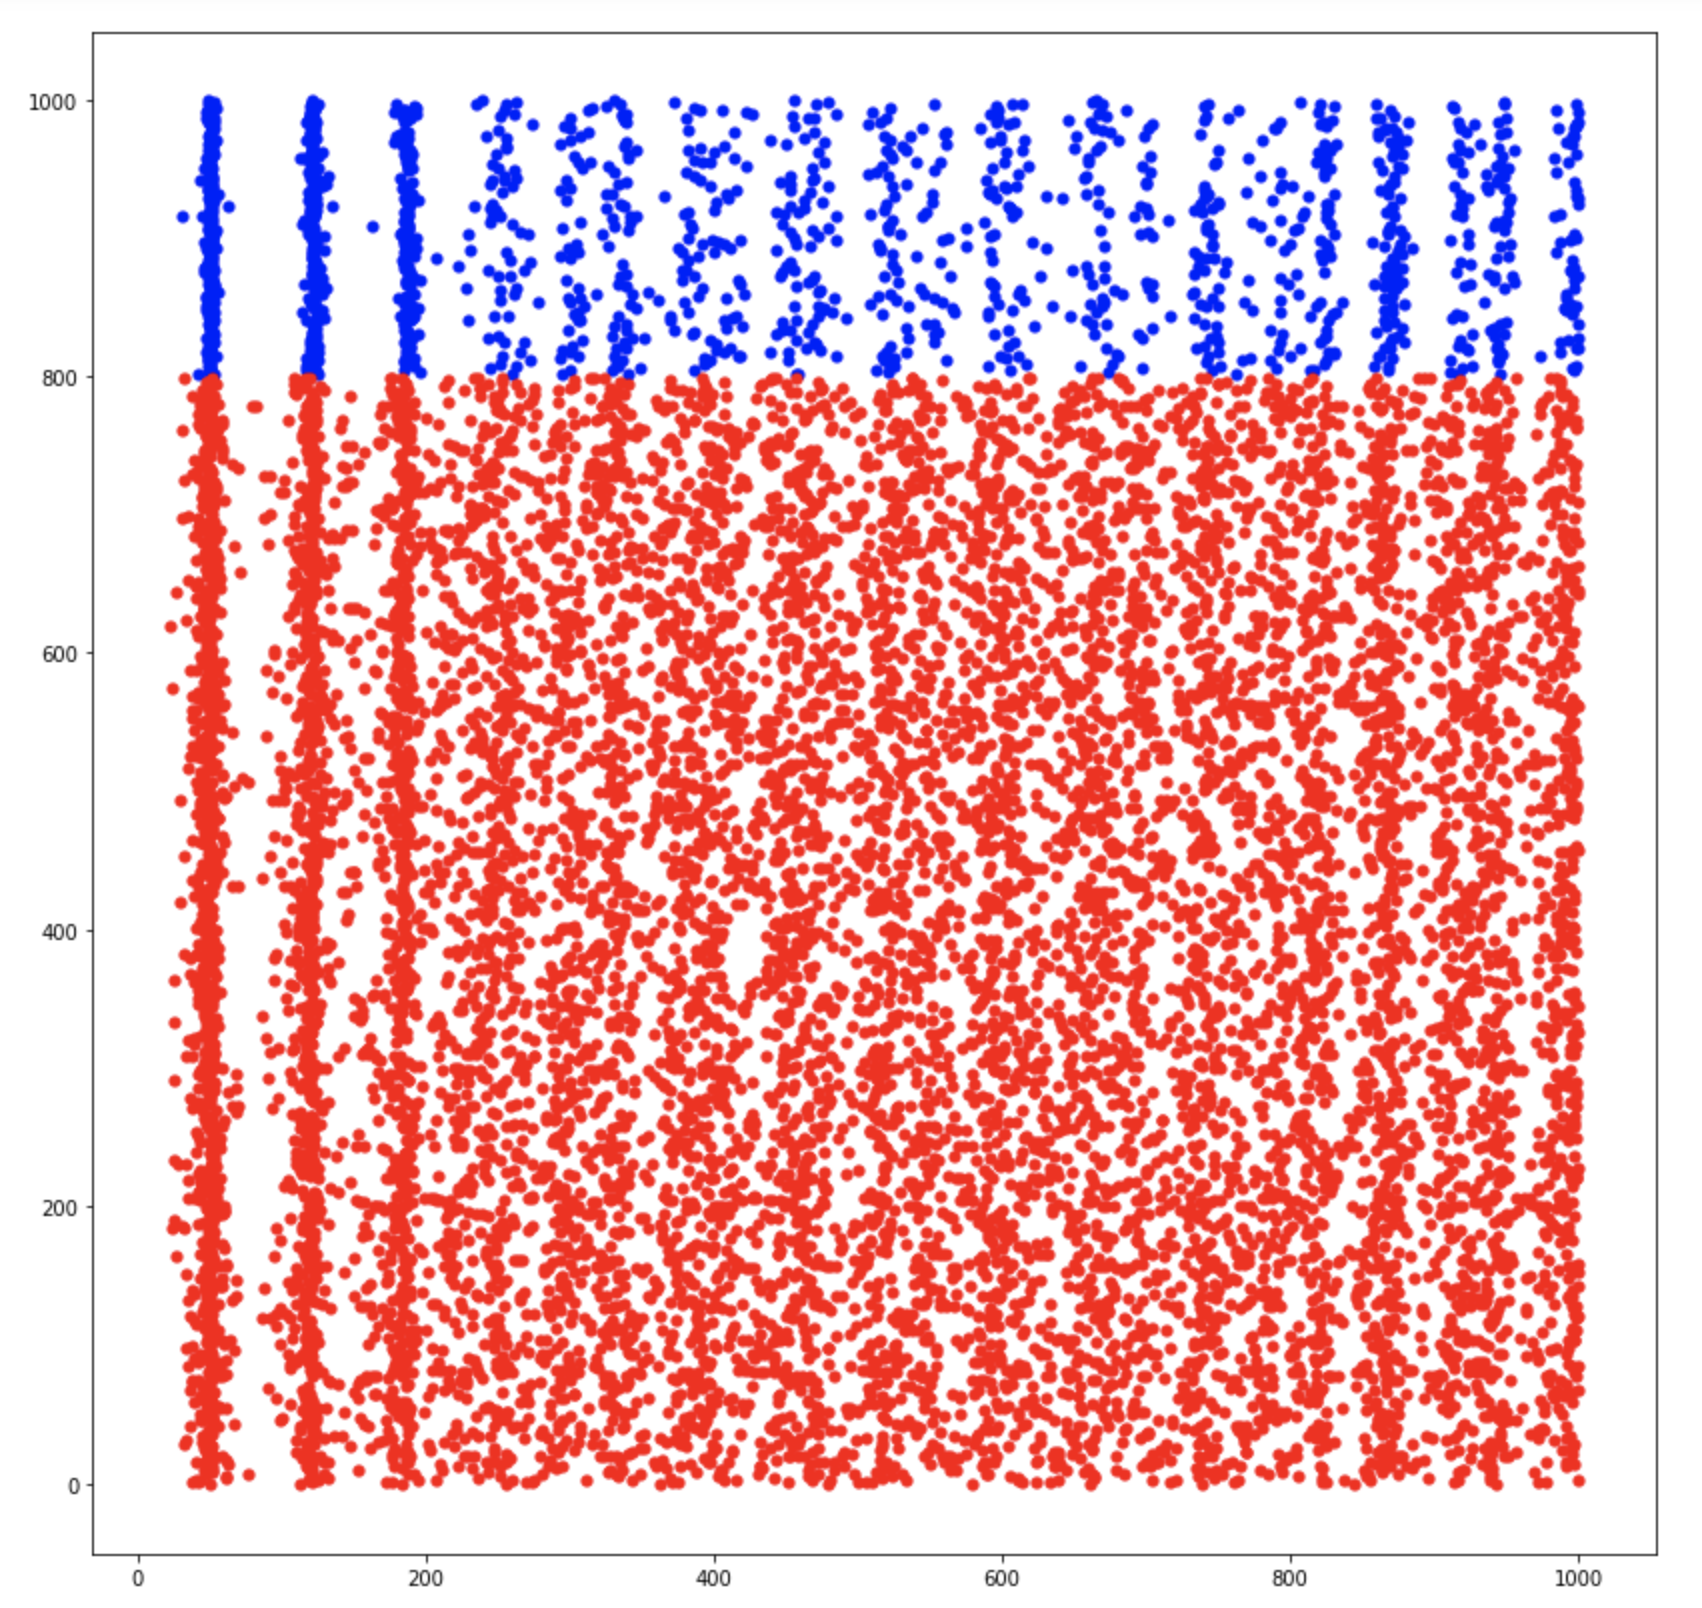
\includegraphics[height=8cm]{images/resultadoSinNorm.png}
    \caption[fontsize=2pt]{Resultado obtenido sin la consideración}.
\end{figure}

\begin{figure}[h!]
    \centering
        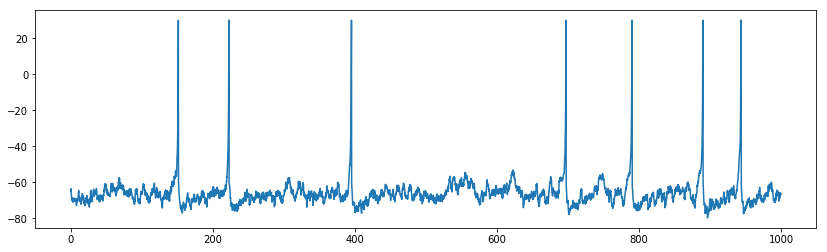
\includegraphics[height=6cm, width=15cm]{images/ejemploNeurona.png}
    \caption[fontsize=2pt]{Ejemplo de $v(t)$ en funcion del tiempo para la neurona 1. El eje X es el tiempo y el Y el potencial de la neurona}.
\end{figure}

\newpage

En ambas figuras (11 y 12) el eje X es el tiempo y el eje Y es el indice de cada neurona. Como se mencionó anteriorimente, el experimento se realizó con 1000 neuronas aleatoriamente conectadas.
Las neuronas azules son las neuronas inhibitorias y las rojas las exitatorias. \\

En ambas imagenes se puede ver que los patrones obtenidos son muy semejantes pero en el segundo caso (figura 12) con ruido que no se encuentra presente en el primer caso.
Esto se podria deber a que al tener la consideración en cuenta al disparar se agrega un estado intermedio entre el disparo y en reset:
\begin{itemize}
    \item Con la consideración: Al hacerse el disparo se setea $v$ en $30$ y en el siguiente instante de tiempo se lo setea en el valor de reset
    \item Sin la consideración: Al hacerse el disparo se setea $v$ directamente al valor de reset.
\end{itemize}

Al agregar un estado mas, le da un tiempo mas a las neuronas vecinas para disparar lo que generaría un patron mucho mas ordenado. \\

A pesar de esta diferencia entre resultados, en ambos se pudo lograr replicar lo obtenido en el paper original que era lograr en una red conectada aleatoriamente disparos sincronizados de las neuronas.
Al igual que en el original, las neuronas inhibitorias son las que mostraron mas claramente la sincronización deseada. Es importante destacar tambien que los disparos no son aleatorios, sino que siguen un ritmo (frecuencia constante). \\

Cambiando la intensidad relativa de las conecciones sinapticas (las conecciones entre neuronas) y la intensidad thalamica hacia cada neurona se pueden reproducir otros tipos de comportamientos
colectivos, incluyendo ondas del huso y oscilaciones del sueño.

Se puede observar y estudiar fácilmente estos estados corticales porque el modelo simple de disparos (el expuesto en el paper original) describe con precisión la dinámica de los tipos conocidos
de neuronas corticales. Por lo tanto, ya no existe un dilema entre la plausibilidad biológica y la eficiencia computacional de las redes neuronales modelo.

\subsection{Simulaciones extras}
A partir de la simulación propuesta por el paper original se hicieron otras simulaciones para intentar generar otras dinámicas.

\subsubsection{Simulacion con doble intensidad}
Para este experimento se duplicó el peso de todas las conecciones entre neuronas al doble. Las inhibitorias eran multiplicadas por un factor de $-1$ el cual paso a $-2$.
El factor de las exitatorias paso de ser $0.5$ a $1$. El resultado obtenido fue el siguiente:

\begin{figure}[h!]
    \centering
        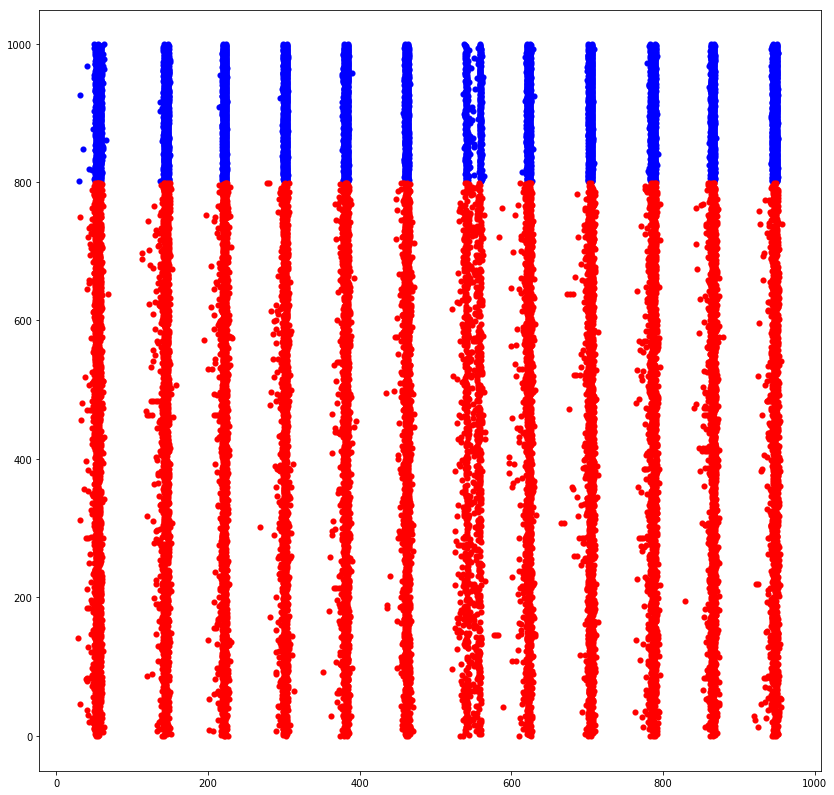
\includegraphics[height=8cm]{images/resultadoDobleAmbos.png}
    \caption[fontsize=2pt]{Resultado obtenido duplicando la intensidad de los pesos de todas las neuronas sin importar el tipo}.
\end{figure}

\newpage

Se puede ver que los disparos estan muy sincronizados, inclusive los de las neuronas exitatorias que era algo que no pasaba en las simulaciones corridas con los parámetros propuestos por el paper.
Tambien se ve claramento que los disparos no son aleatorios si no que siguen un ritmo (tienen aparentemente una frecuencia constante).

\subsubsection{Simulación intensificando distintos tipos de neuronas}
Para este experimento se hicieron dos simulaciones:
\begin{itemize}
    \item Cuadriplicando el factor multiplicador de las neuronas exitatorias por cuatro: pasó de $0.5$ a $2$, dejando por default el multiplicador de las inhibitorias. Figura 16.
    \item Cuadriplicando el factor multiplicador de las neuronas inhibitorias por cuatro: pasó de $-1$ a $-4$, dejando por default el multiplicador de las exitatorias. Figura 15.
\end{itemize}

\begin{figure}[htp!]
    \centering
        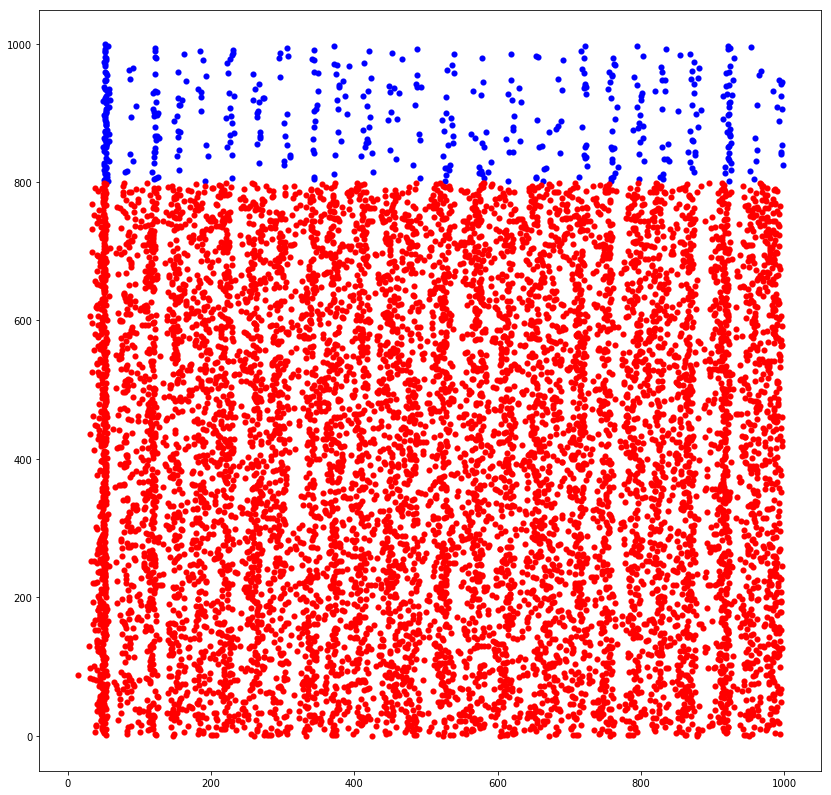
\includegraphics[height=8cm]{images/resultadoCuadrupleInhibitoria.png}
    \caption[fontsize=2pt]{Resultado obtenido cuadriplicando el factor de multiplicación del peso de las inhibitorias}.
\end{figure}


\begin{figure}[htp!]
    \centering
        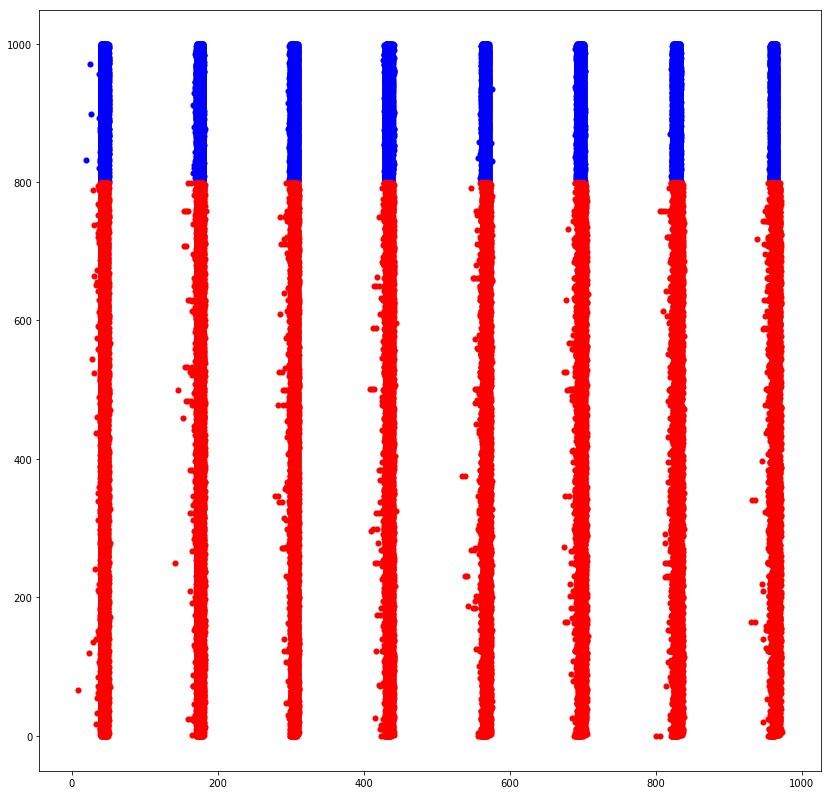
\includegraphics[height=8cm]{images/resultadoCuadrupleExitatorias.png}
    \caption[fontsize=2pt]{Resultado obtenido cuadriplicando el factor de multiplicación del peso de las exitatorias}.
\end{figure}

\begin{figure}[htp!]
    \centering
        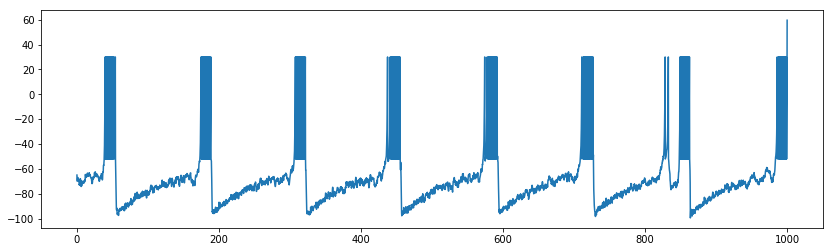
\includegraphics[height=6cm, width=15cm]{images/ejemploNeuronaCuadrupleExitatoria.png}
    \caption[fontsize=2pt]{Ejemplo de $v(t)$ en funcion del tiempo para la neurona 1 para el caso que se cuadriplica el factor del peso de las exitatorias}.
\end{figure}

\newpage

Se pueden sacar varias conclusiones a partir de la comparación entre ambas simulaciones y en comparación a las simulaciones previamente realizadas:
\begin{itemize}
    \item En la figura 15 se ve un ritmo con mucha menor frecuencia y con mucho mas ruido, entonces podemos concluir que es la intensidad de las exitatorias (que en esta simulación era el por defecto)
    la que hace una mejor sincronizacion entre las neuronas. Es importante aclarar que en este caso las inhibitorias son las que tienen mas intensidad de lo normal y eso podria ser lo que genera el ruido.
    \item Se puede ver en la figura 16 que al hacer mas intensas a las exitatorias, el ritmo de las neuronas es mucho mas claro y ademas tiene un frecuencia mayor a la original (figura 11).
    \item En la figura 17, que es una neurona exitatoria del experimento de la figura 16, se ve que las neuronas pasan a tener un comportamiento mas parecido a una neurona del tipo CH y no tanto RS, que es el comportamiento mas comun en el experimento original (se puede comparar con la figura 13).
\end{itemize}

\subsubsection{Comportamientos no esperados}
Es importante mencionar que no siempre se pudieron generar las imagenes deseadas. Hubo casos para los cuales la aleatoriedad de los pesos no le dió suficente intensidad a las neuronas exitatorias haciendo que haya realmente muy pocos disparos.
En la figura 18 se puede ver uno de esos casos.

\begin{figure}[htp!]
    \centering
        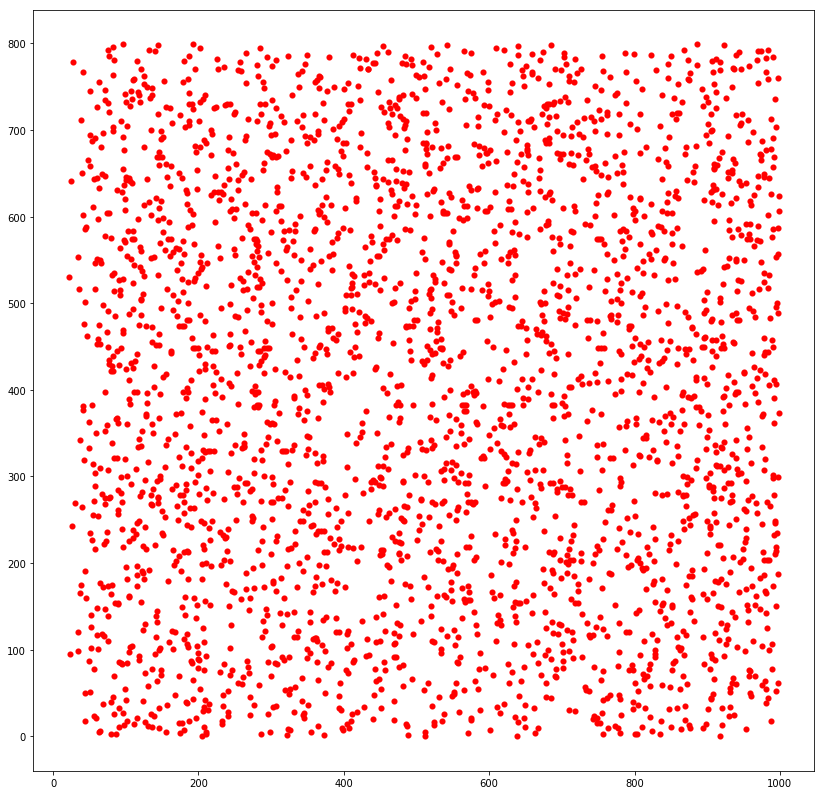
\includegraphics[height=8cm]{images/resultadoVacio.png}
    \caption[fontsize=2pt]{Resultado con pocos disparos. En la figura se puede ver que el eje Y que llega hasta 800, lo que significa que las neuronas que van del 801 al 1000 (las inhibitorias) no dispararon nunca}.
\end{figure}

\newpage

Se puede ver en el grafico que las únicas neuronas que disparon fueron las exitatorias.
Hay una cantidad mucho menor de disparos comparado con un escenario normal como el de la figura 12 por ejemplo.
Es un caso que se genera aproximadamente una de cada cuatro simulaciones.

\newpage

\section{Bonus: Nest}

Con la intención de aprender otra herramienta mas, se intentó utilizar la libreria $Nest$ \cite{Nest}. Esta herramienta provee un monton de modelos neuronales ya armados con los cuales se pueden simular muchisimas dinámicas de distintos tipos de neuronas.
Dependiendo los requerimientos se pueden usar modelos muy complejos o muy simples.
$Nest$ resuelve las ecuaciones diferenciales dejando al usuario la única tarea de definir los parámetros del modelo requerido.
Tambien, el modelo provee varias herramientas para medir distintas variables en simultaneo de los modelos a travez del tiempo.
La libreria dispone del modelo de este paper (en la clase $izhikevich$ \cite{nest_izhikevich}) por lo que se utilizo para modelar dos de las neuronas simuladas en este paper: RS y CH.

\begin{figure}[h!]
    \centering
        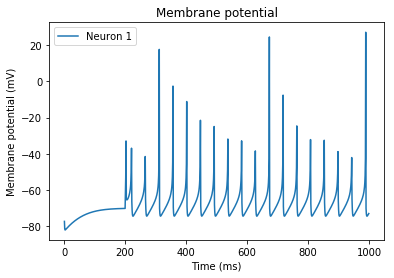
\includegraphics[height=8cm]{images/RS_nest.png}
    \caption[fontsize=2pt]{Resultado obtenido usando $Nest$ con los parámetros de la neurona RS. Se puede comparar con la figura 2}.
\end{figure}

\begin{figure}[h!]
    \centering
        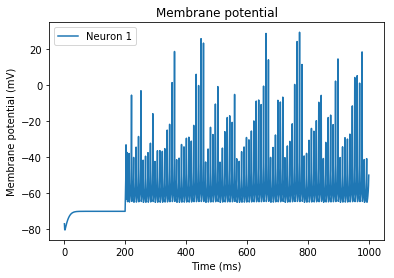
\includegraphics[height=8cm]{images/CH_nest.png}
    \caption[fontsize=2pt]{Resultado obtenido usando $Nest$ con los parámetros de la neurona CH. Se puede comparar con la figura 5}.
\end{figure}

\newpage

Se puede concluir que los resultados fueron semejantes a los de las simulaciones realizadas en este paper (y en el original) con la diferencia del voltaje máximo de los disparos.
En los simulados con $Nest$ se puede ver que los disparos varian mucho su voltaje máximo (van desde $-40$ hasta $30$) a diferencia de los del paper original que tenian un voltaje maximo con mucha menor varianza (desde $10$ hasta $30$).
Esto se puede deber a modificaciones realizadas en la libreria $Nest$ para ajustar aun mas el modelo de $izhikevich$, esos ajustes se pueden ver en \cite{nest_izhikevich}.

\newpage

\section{Conclusiones}

Se pudó probar que el modelo simple propuesto en el paper reproduce el comportamiento de neuronas biológicas, incluyendo los disparos, los estallidos y mezclas de patrones. El paper propone que ese modelo es el modelo mas simple posible que puede reproducir el comportamiento de todas estas neuronas.
Solo consiste en dos eucuaciones y tiene solo un elemento no lineal ($v(t)^2$).
Aun asi, el modelo es canonico en el sentido de que la diferencia entre el mismo y toda la clase de modelos biofísicamente detallados y precisos de tipo Hodgkin-Huxley, incluyendo los que tienen una cantidad enorme de ecuaciones y tienen en cuenta mucha mas información es solo un tema de cambio de coordenadas. \\

Se mostró como usar el modelo para generar redes de neuronas capaces de reproducir dinámicas y ritmos colectivos similares a los que se producen en un cortex de un mamifero.
Al ser el modelo extremadamente simple computacionalmente, se puede usar para simular redes thalamicas-corticales que contengan miles y miles de neuronas en tiempo real con resolución de $1 ms$. \\

Como conlución de la simulación del paper original: Se puedieron replicar todos los casos mencionados en el mismo con las dificualtades ya mencionadas anteriormente este documento.
Ademas se realizaron simulaciones con parámetros distintos a los originales para intentar generar nuevos patrones.
Finalmente se aprendió a usar una libreria ya existente y muy utilizada para la simulación de neuronas.
A la vez, la realización de la simulación de este paper (y seguramente de cualquier otro) dió al autor de este documento una introducción a las publicaciones cientificas y a sus formatos, que no es algo muy comun
a lo largo de la carrera.
El autor de este documento recomienda fuertemente esta experiencia ya que le fue sumamente enriquecedora.

\section{Repositorio}
Todos los experimentos fueron realizados con el código que se puede encontrar en el siguiente repositorio: \\
\url{https://github.com/fedebrasburg/simple-model-of-spiking-neurons}

\newpage

\section{Referencias}

\begin{thebibliography}{9}

\bibitem{paperOriginal}
Izhikevich
\textit{Simple Model of Spiking Neurons}. (Ingles) 2003

\bibitem{HodgkinHuxley}
Martin Pospischil. Maria Toledo-Rodriguez. Cyril Monier. Zuzanna Piwkowska. Thierry Bal. Yves Frégnac. Henry Markram
\textit{Minimal Hodgkin–Huxley type models for different classes of cortical and thalamic neurons}. (Ingles) 2008

\bibitem{modeloPrimero}
Int. J. Bifurc.
\textit{Neural excitability, spiking and bursting}. (Ingles) 2000

\bibitem{bifurcacion}
E. M. Izhikevich.
\textit{Dynamical Systems in Neuroscience: The Geometry of Excitability and Bursting}. (Ingles) A ser publicado

\bibitem{Euler}
Euler.
\textit{Método de Eurler}. \url{https://en.wikipedia.org/wiki/Euler_method}

\bibitem{Sympy}
\textit{Sympy}. \url{https://docs.sympy.org/latest/index.html}

\bibitem{firingPatters}
B. W. Connrs y M. J Gutnick.
\textit{Intrinsic firing patterns of diverse neocortical neurons}. (Ingles) Trends in Neurosci., vol. 13, pp. 99-104, 1990.

\bibitem{chatteringCells}
C. M. Gray y D. A. McCormick.
\textit{Chattering cells: superficial pyramidal neurons contributing to the generation of synchronous oscillations in the visual cortex}. (Ingles) Science. vol 274, no. 5284, pp 109-113, 1996.

\bibitem{inhibitorias}
J. R. Gibson, M. Belerlein, and B. W. Connors,
\textit{Two networks of elec- trically coupled inhibitory neurons in neocortex}. (Ingles) Nature, vol. 402, pp. 75–79, 1999.

\bibitem{saddleNode}
\textit{Neural excitability, spiking, and bursting}. (Ingles) Int. J. Bifurc. Chaos, vol. 10, pp. 1171–1266, 2000.

\bibitem{MatLab}
\textit{MatLab}. \url{https://www.mathworks.com/products/matlab.html}

\bibitem{Python}
\textit{Python}. \url{https://www.python.org/}

\bibitem{Nest}
\textit{Nest}. \url{https://www.nest-simulator.org/}

\bibitem{nest_izhikevich}
\textit{izhikevich - Nest}. \url{https://www.nest-simulator.org/helpindex/cc/izhikevich.html}

\end{thebibliography}

\end{document}
